\clearpage{\pagestyle{empty}\cleardoublepage}
\chapter{Moto dei fluidi nelle condotte in pressione}\label{ch:fluidodinamica}
\chaptermark{Fluidi in condotta}
La fluidodinamica è un ramo della meccanica del continuo e studia il comportamento di liquidi e gas in movimento. Si parla di termofluidodinamica quando, in alcuni processi, le grandezze e i fenomeni termici sono particolarmente rilevanti. Lo studio del moto dei fluidi in condotta riveste notevole importanza nella progettazione di qualsiasi impianto industriale, dove il calcolo delle perdite di carico rappresenta il nodo cruciale per un'appropriata interpretazione e risoluzione del problema. Solitamente in ambito tecnico non si fa riferimento a fluidi monofase, bensì a fluidi multifase, dove l'iterazione tra fasi gioca un ruolo fondamentale e il calcolo delle variabili è possibile solo grazie a modelli complessi e fortemente dipendenti dalle condizioni al contorno. 
\section{Il concetto di fluido e nozioni fondamentali}
Per fluido si intende un materiale che non è in grado di reagire a sforzi di taglio statici. Non si trasmettono quindi, in condizioni di quiete, forze parallele attraverso una qualunque superficie ideale tracciata nel fluido. Attraverso la stessa superficie possono trasmettersi forze perpendicolari, la cui risultante è nota come \textit{pressione}.\\
La densità di un fluido \(\rho\) è definita come la massa dell'unità di volume. Si definisce densità relativa \(\rho_r\) il rapporto tra la densità del materiale e quella dell'acqua a pressione atmosferica e temperatura a 4°C. Il peso specifico \(\gamma\) è il peso dell'unità di volume. Per volume specifico \(v\) si intende il volume dell'unità di massa, cioè l'inverso della densità. \\
In condizioni dinamiche un fluido, al contrario delle condizioni di quiete, reagisce a sforzi di taglio. Si consideri un meato (intercapedine in cui è presente un piccolo strato di fluido) di altezza \(h\), delimitato tra due pareti piane indefinite, una in quiete e l'altra in movimento con velocità \(w\) (\figref{fig:meato}).
\begin{figure}[htbp] %Immagine meato
    \centering
    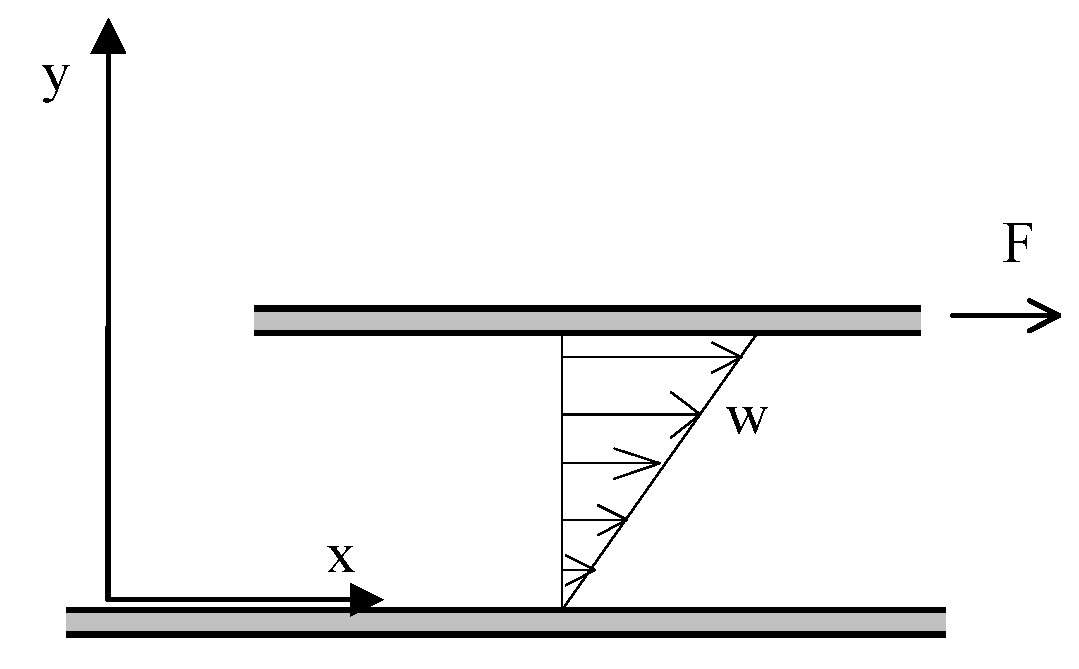
\includegraphics[width=0.6\textwidth]{fig/fluidodinamica/meato.eps}
    \caption{Azioni esercitate da un fluido tra due superfici in moto relativo \parencite{guglielmini2004lezioni}.} 
    \label{fig:meato}
\end{figure}
Il moto relativo tra fluido e parete è nullo, nel meato si crea quindi un campo di velocità triangolare, dove i piani di fluido scorrono l'uno sull'altro. Questo genera una forza resistente sulla superficie della parete superiore in moto. Indicando con \(A\) l'area della superficie di contatto tra  la lastra e il fluido, la forza resistente \(F\) è espressa in modulo dalla legge di Newton:
\[F= \mu \; A \; \frac{dw}{dy} \implies \tau_{yx} = \frac{F}{A} = \mu \; \frac{dw}{dy} \addtag \label{eq:newton} \]
in cui \(\mu\) è una proprietà del fluido detta viscosità dinamica e \(\tau_{yx}\) rappresenta lo sforzo di taglio viscoso ovvero la forza che agisce per unità di area su  una superficie interna al fluido in direzione parallela a tale superficie, e \(\frac{dw}{dy}\) è la derivata della velocità del fluido rispetto alla componente verticale del moto. Lo sforzo di taglio è proporzionale alla viscosità e al gradiente di velocità. Il rapporto è direttamente proporzionale se i fluidi sono classificabili come newtoniani, cioè se la viscosità è indipendente dallo sforzo viscoso per determinate condizioni di temperatura e pressione. Per i fluidi non newtoniani vale la seguente formula:
\[\frac{dw}{dy}=\frac{\tau}{\mu(\tau)}\addtag\label{eq:newtoniani}\]
A seconda dell'andamento della funzione \(\mu(\tau)\) i fluidi possono essere classificati come "pseudo plastici" o "dilatanti" (\figref{fig:newtoniani}).
\begin{figure}[htbp] %Immagine reologia di un fluido
    \centering
    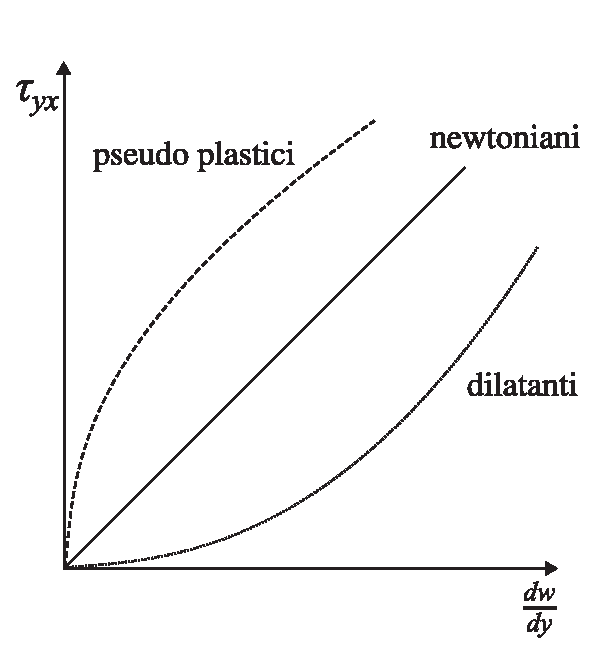
\includegraphics[width=0.5\textwidth]{fig/fluidodinamica/newtoniani.eps}
    \caption{Reologia di un fluido nel caso di fluidi newtoniani e non newtoniani \parencite{guglielmini2004lezioni}.} 
    \label{fig:newtoniani}
\end{figure}
\section[Moto e equazioni fondamentali]{Schematizzazione del moto e equazioni fondamentali di conservazione}
\sectionmark{Moto e equazioni fondamentali}
La rappresentazione analitica del moto di un fluido è assai complessa e richiede l'impiego di modelli al fine di semplificare la descrizione qualitativa e quantitativa di tale moto. Vengono indicate le tre figure fondamentali per la descrizione del moto di un fluido:
\begin{itemize}
\item \textbf{traiettoria di una particella}: il luogo dei punti occupati in tempi successivi dalla stessa particella fluida;
\item \textbf{linea di corrente} o \textbf{linea di flusso}: è una linea che ha per tangente il vettore velocità in ogni punto;
\item \textbf{linea di fumo}: è il luogo dei punti occupati, ad un dato istante, dalle particelle che sono passate per uno stesso punto.
\end{itemize}
Nel caso di moto permanente questi  tre luoghi geometrici coincidono. Si definisce vena fluida o filetto di corrente l'insieme delle traiettorie le cui sezioni trasversali hanno velocità (perpendicolare alla sezione stessa), pressione, temperatura e volume specifico costanti.\\
Il modello di riferimento è quello di moto uni- o monodimensionale e si assumono condizioni di regime permanente di massa e termodinamico. In termini fisici il modello deve rispettare i principi di:
\begin{itemize}
\item \textbf{conservazione della massa};
\item \textbf{conservazione della quantità di moto};
\item \textbf{bilancio di energia}.
\end{itemize}

\paragraph{Conservazione della massa}
Dato un sistema di coordinate cartesiane (x, y, z), si consideri un volume di controllo (VC) con gli spigoli \(dx\), \(dy\), \(dz\), attraversato da un fluido con velocità \(w\) e densità \(\rho\) (\figref{fig:vc}). Siano \(w_x\), \(w_y\) e \(w_z\) le componenti del vettore velocità lungo gli assi principali. Si definisce \(j\) velocità di massa o flusso di massa e si calcola la portata massica in entrata e in uscita sul VC lungo le tre direzioni principali. Se si sommano queste portate, si esprime la variazione di massa infinitesima \(dm\) nel tempo infinitesimo \(dt\) relativa al VC:
\[dm= - \left[\dfrac{\partial(\rho \; w_x)}{\partial x} + \dfrac{\partial(\rho \; w_y)}{\partial y} + \dfrac{\partial(\rho \; w_z)}{\partial z} \right]dx \; dy \; dz \; dt \label{eq:conservazione} \addtag \]
La massa di VC può essere espressa anche come il prodotto della densità del fluido per il volume :
\[m= \rho \; dx \; dy \; \label{eq:massa}\ \addtag \]
e la variazione nel tempo è:
\[dm = \dfrac{\partial}{\partial t}\rho \; dx \; dy \; dz \label{eq:varmassa} \addtag \]
Per il principio di conservazione della massa, la \eqref{eq:conservazione} e la \eqref{eq:varmassa} devono equivalersi:
\[\dfrac{\partial(\rho \; w_x)}{\partial x} + \dfrac{\partial(\rho \; w_y)}{\partial y} + \dfrac{\partial(\rho \; w_z)}{\partial z}= - \dfrac{\partial \rho}{\partial t} \addtag \label{eq:continuita} \]
La \eqref{eq:continuita} rappresenta l'equazione di continuità di un fluido in coordinate cartesiane e può essere anche essere scritta come:
\[ \vec{\nabla} (\rho \vec{w}) = -\dfrac{\partial \rho}{\partial t} \addtag \label{eq:continuitadiff} \]

\begin{figure}[htbp] 
    \centering
    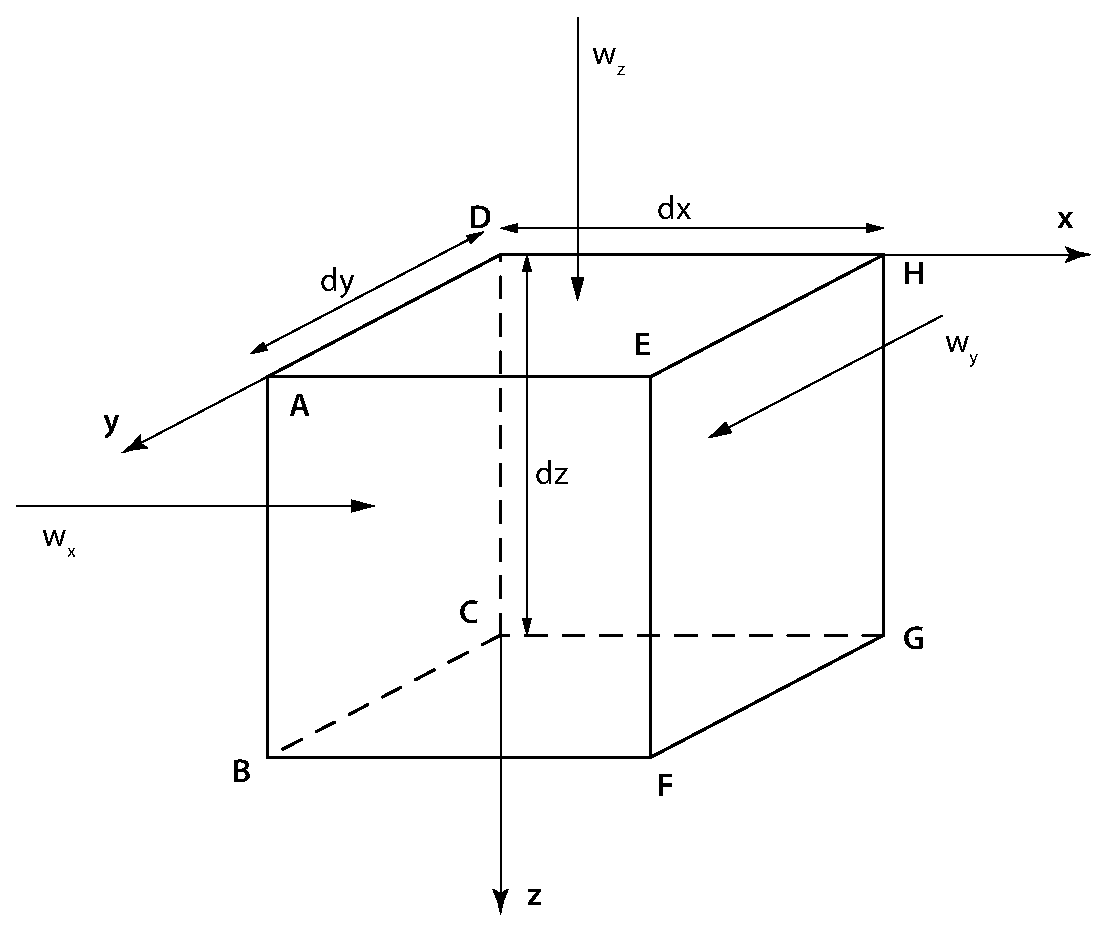
\includegraphics[width=.5\textwidth]{fig/fluidodinamica/cv.eps}
    \caption{Schematizzazione del parallelepipedo fondamentale o volume di controllo (VC).} 
    \label{fig:vc}
\end{figure}

\paragraph{Bilancio della quantità di moto}
La conservazione della quantità di moto è espressa dal secondo principio della dinamica. Dato un volume di controllo VC (definito precedentemente)la somma della variazione nel tempo \(dt\) della quantità di moto del fluido di volume \(V\)e del flusso netto di quantità di moto attraverso la superficie \(S\) è uguale alla risultante delle forze esterne agenti sul fluido contenuto nel volume stesso.
In forma integrale:
\[\frac{d}{dt} \int_V \rho \vec w \, dV + \oint_S \left( \rho \vec w \right) \vec w \cdot \hat n \, dS = \int_V \vec F_V \, dV + \oint_S \underline{\underline T } \addtag \label{eq:intconsqm} \]
dove \(\underline{\underline T }\) rappresenta il tensore delle tensioni, \(\hat n\) il relativo versore e \(\vec F_V\) le forze di volume. In forma differenziale la \eqref{eq:intconsqm} diventa:
\[\rho \frac{D \vec u}{Dt} = \rho \vec F_V + \nabla \cdot \underline{\underline T } \addtag \]
che esprime il bilancio della quantità di moto per unità di volume.


\paragraph{Bilancio di energia e equazione di Bernoulli}
Tra le sezioni estreme di una generica vena fluida si applica l'equazione di bilancio dei sistemi aperti a regime permanente. Si considera come VC il volume racchiuso tra le due sezioni sopra citate. L'equazione di bilancio per unità di massa di un sistema aperto si può scrivere in forma differenziale come:
\[dQ-dL_e=dH+\frac{dw^2}{2}+gdz\addtag\]
dove $dQ$ e $dL_e$ rappresentano rispettivamente il calore scambiato con l'ambiente esterno e di lavoro esterno netto attraverso la superficie di confine, $dH$ rappresenta l'entalpia, $z$ la quota potenziale e \(g\) la costante di gravitazione universale (\(g \simeq 9,81\) m/s\ap{2}). Poiché $dh=TdS_s+vdp$:
\[dL_e+TdS_s+v \; dp+\frac{dw^2}{2}+g \; dz\label{eq:intermediobernoulli}\addtag\]
dove $dS_s$ è la produzione entropica elementare e $v$ il volume specifico. Un qualunque lavoro specifico, può essere espresso come prodotto di un volume specifico per un'opportuna pressione differenziale $dp'$, per omogeneità dimensionale. Questa variazione di pressione differisce dalla variazione che il fluido subisce in moto. Sapendo che una qualsiasi pressione $p$ può essere espressa in termini di peso specifico $\gamma$ e altezza idrica $h$:
\[dL_e=v\;dp_e=v\;\gamma\;dh_e=g\;dh_e\addtag\label{eq:lavoroesterno}\]
Allo stesso modo per il lavoro di attrito:
\[dL_a=v\;dp_a=v\;\gamma\;dh_a=g\;dh_a\addtag\label{eq:lavoroattrito}\]
Se sostituiamo la \eqref{eq:lavoroesterno} e la \eqref{eq:lavoroattrito} nella \eqref{eq:intermediobernoulli} otteniamo:
\[dh_e+dh_a+\frac{dp}{\gamma}+\frac{dw^2}{2g}+dz=0\label{eq:bernoulligeneralizzata}\addtag\]
La \eqref{eq:bernoulligeneralizzata} è detta equazione di Bernoulli generalizzata in forma differenziale e ha valenza energetica specifica (per unità di peso). I termini nella formula sono così nominati:
\begin{itemize}
    \item \(\mathbf{dh_e}\) \textbf{carico motore}, termine effettivo di scambio con l'esterno;
    \item \(\mathbf{dh_a}\) \textbf{carico d'attrito}, termine di dissipazione;
    \item \(\mathbf{\dfrac{dp}{\gamma}}\) \textbf{carico piezometrico}, l'effettiva variazione di pressione del fluido dovuta al moto;
    \item \(\mathbf{\dfrac{dw^2}{2g}}\) \textbf{carico cinetico};
    \item \(\mathbf{dz}\) \textbf{carico gravitazionale}, variazione di quota geodetica. 
\end{itemize}
Se la \eqref{eq:bernoulligeneralizzata} viene integrata tra la sezione 1 e la sezione 2 si ottiene:
\[(h_e)_{1,2}+(h_a)_{1,2}+\int^2_1{\frac{dp}{\gamma}}+\frac{w^2_2-w^2_1}{2g}+z_2-z_1=0\label{eq:bernoulliintegrata}\addtag\]
L'equazione caratterizzante il moto è così ridotta in termini di carichi differenziali, cioè in termini dimensionali si hanno delle lunghezze.\\
In caso di un condotto a pareti rigide, di sezione costante, orizzontale e attraversato da un fluido a regime permanente, cioè a carico motore e potenziale nullo, la \eqref{eq:bernoulliintegrata} diventa:
\[(h_a)_{1,2}+\int^2_1{\frac{dp}{\gamma}}+\frac{w^2_2-w^2_1}{2g}=0\label{eq:attritointermedio}\addtag\]
Se si ammettono trascurabili le variazioni di peso specifico rispetto alle variazioni di pressione, cioè si assume che il peso specifico sia costante, e la variazione di velocità nulla:
\[(h_a)_{1,2}=\frac{p_1-p_2}{\gamma}\label{eq:caricoattrito}\addtag\]
La \eqref{eq:caricoattrito} esprime il carico d'attrito o in termini operativi la perdita di carico. 
%%%%%%%%%%%%%%%%%%%%%%%%%%%%%%%%%%%%%%%%%%%%%%%%%%%%%%%%%%%%%%
\section{Calcolo delle cadute di pressione per attrito}
\subsection{Numero di Reynolds}
Si consideri un condotto rettilineo a pareti perfettamente lisce in cui scorre un fluido a velocità \(w\), di densità \(\rho\) e viscosità \(\mu\). Il regime è definito laminare se le traiettorie del flusso sono rettilinee e il profilo di velocità è parabolico (\figref{fig:laminare}). Il regime di flusso è invece turbolento quando le particelle non seguono traiettorie ordinate e il moto che ne risulta avviene in maniera caotica (\figref{fig:turbolento}).

\begin{figure}[htbp]
\centering
    \subfloat[][Moto laminare]
    {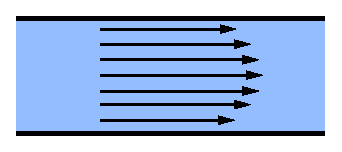
\includegraphics[width=.4\textwidth]{fig/fluidodinamica/laminareturbolento/laminare.eps} \label{fig:laminare}} \qquad \qquad
    \subfloat[][Moto turbolento]
    {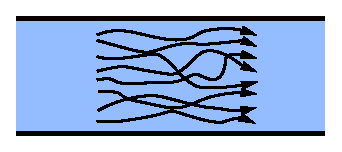
\includegraphics[width=.4\textwidth]{fig/fluidodinamica/laminareturbolento/turbolento.eps} \label{fig:turbolento}} \\
\caption{Regime di flusso monofase in condotta.}
\label{fig:laminareturbolento}
\end{figure}

Reynolds fu il primo a definire che il tipo di moto dovesse dipendere non solo dalla velocità ma anche dalla densità e viscosità del fluido oltre che alla geometria della condotta. Il numero di Reynolds è così definito:
\[Re=\frac{\rho \; w \; D}{\mu}\addtag\label{eq:reynolds}\]
Il numero di Reynolds definisce il tipo di moto che si instaura in condotta:
\begin{itemize}
    \item per \(Re<2000\qquad\)il moto in un condotto è laminare;
    \item per \(2000<Re<10000\qquad\)si ha una regione di transizione;
    \item per \(Re>10000\qquad\)il moto in un condotto è completamente turbolento.
\end{itemize}
%%%%%%%%%%%%%%%%%%%%%%%%%%%%%%%%%%%%%%%%%%%%%%%%%%%%%%%%%%%%%%
\subsection{Fattore di attrito di Moody}
Sia in condizioni di moto laminare che, in condizioni di moto turbolento, la caduta di pressione totale dipende dal tipo di fluido, dal regime di moto e dalle caratteristiche della condotta. In breve, il carico di attrito dipende da parametri:
\begin{itemize}
    \item \textbf{fisici} - \(\mu\) e \(\rho\) - relativi ai fluidi in movimento;
    \item \textbf{cinematici} - \(w\) - caratterizzanti il trasporto di massa fluida;
    \item \textbf{geometrici} - \(D\) e \(\epsilon\) - legati alla tubazione e alla \textit{scabrezza assoluta} della parete interna della condotta.
\end{itemize}
Perciò si può affermare che:
\[\frac{\Delta p}{l}=f(\rho, \; \mu, \; w, \; D, \; \epsilon) \addtag \label{eq:funzcaduta} \]
dove \(l\) è la lunghezza della condotta. L'equazione di Darcy-Weisbach può essere definita sia in funzione delle perdite di carico piezometriche \eqref{eq:darcyweisbachH} sia in funzione delle cadute di pressione \eqref{eq:darcyweisbachP}:
\[h_a = \lambda \; \frac{l}{D} \; \frac{w^2}{2 \; g} \addtag \label{eq:darcyweisbachH} \]
\[\Delta p_a = \lambda \; \frac{l}{D} \; \frac{\rho \; w^2}{2} \addtag \label{eq:darcyweisbachP} \]
dove \(\lambda\) è detto \textit{fattore d'attrito di Moody} o \textit{indice di resistenza}. La perdita di carico corrispondente, per un certo valore \(\lambda\), risulta proporzionale al carico cinetico e alla lunghezza del condotto. In regime di moto laminare il fattore di attrito è proporzionale al solo coefficiente di Reynolds:
\[\lambda=\frac{64}{Re} \addtag \]
In regime tubolento l'indice di resistenza è legata alla rugosità della parete. Il rapporto \(\frac{\epsilon}{D}\) è definito \textit{scabrezza relativa}. La relazione funzionale equivalente è:
\[\lambda=f \; \left(Re, \; \frac{\epsilon}{D}\right) \addtag \]
Sulla base dei risultati sperimentali al variare dei parametri del modello di flusso in condotta in regime turbolento, è stato costituito il \textit{diagramma di Moody} (\figref{fig:moody}). Gli andamenti all'interno di tale diagramma sono la rappresentazione grafica della \textit{correlazione di Colebrook}:
\[ \frac{1}{\sqrt{\lambda}} = - 2 \ln \left( \frac { \epsilon/D} {3{,}71} + \frac {2{,}51} {Re \, \sqrt{\lambda}} \right) \addtag \label{eq:colebrook} \]

\begin{figure}[htbp] %Immagine diagramma di Moody
    \centering
    \includegraphics[width=.9\textwidth]{fig/fluidodinamica/moody.eps}
    \caption{Diagramma di Moody per il calcolo del fattore di attrito in condotta.} 
    \label{fig:moody}
\end{figure}

Il fattore di attrito può essere espresso anche tramite il \textit{numero di Fanning} \(f\), adimensionale e definito come il rapporto tra gli sforzi di taglio e le forze di inerzia:
\[f=\dfrac{2\tau}{\rho w^2} \addtag \label{fanning} \]
Il fattore di attrito di Moody è quattro volte il numero di Fanning:
\[\lambda = 4f \addtag \label{eq:fanningmoody} \]
Blasius propone il calcolo del numero di Fanning a partire dal numero di Reynolds:
\[f=\dfrac{0,079}{Re^{0,25}} \addtag \label{eq:fanningreynolds} \]
La \eqref{eq:fanningreynolds} è applicabile in condizione di tubi a pareti interne lisce (scabrezza nulla, \(\epsilon=0\)) e regime di flusso non totalmente turbolento (\(Re<10^5\)).
%%%%%%%%%%%%%%%%%%%%%%%%%%%%%%%%%%%%%%%%%%%%%%%%%%%%%%%%%%%%%%%%%%%%%%
\subsection{Perdite di carico per un liquido}
Una relazione approssimativa per la valutazione delle perdite di carico di liquidi in condotta è quella di Hazen-Williams.  Questa relazione è valida solo per acqua in condizioni di regime turbolento a temperatura compresa tra i 4°C e 25°C.
\[\frac{h_a}{l} = \frac{10,65\ Q^{1,85}}{C^{1,85}\ d^{4,87}} \addtag \label{eq:HW}\]
dove \(Q\) è la \textit{portata volumetrica}, la costante moltiplicativa numerica 10,65 non è adimensionale (ha le dimensioni di \(s^{1,85}/m^{0,86}\)) e la costante adimensionale \(C\) è un valore tabellato.
\begin{table}[htbp]
    \small
    \centering
    \begin{tabular}{|l|r|}
        \hline
        \textbf{Tipologia tubo} & \(\mathbf{C}\)\\
        \hline
             Tubi estremamente lisci & 140\\
        Tubi nuovi, acciaio o ghisa & 130\\
        Tubi in legno o calcestruzzo & 120\\
        Tubi in acciaio rivettato, nuovi & 110\\
        Tubi vecchi in ghisa, mattoni & 100\\
        Tubi in acciaio rivettato, vecchi & 95\\
        Tubi in acciaio corroso & 80\\
        Tubi in acciaio fortemente corroso & 60\\
        \hline
    \end{tabular}
    \label{tab:coefficientiHZ}
    \caption{Coefficienti $C$ adimensionali per la formula di Hazen-Williams.}
\end{table}
L'equazione fornisce direttamente il valore delle perdite di carico distribuite per unità di lunghezza della tubazione in funzione della portata volumetrica e del diametro idraulico. Se ora esplicitiamo la \eqref{eq:darcyweisbachH} in funzione del diametro interno \(D\), ponendo la \textit{portata volumetrica} come \(Q=w \, A\):
\[h_a = \lambda \; \frac{l}{D} \; \frac{w^2}{2 \; g} \quad \implies \quad \frac{h_a}{l}=\frac{8 \, f}{\pi^2 \, 2g} \, \frac{Q^2}{D^5} \addtag \label{eq:darcyweisbachespl} \]
In entrambe le formulazioni (la forma generale delle perdite di carico e l'apporssimazione di Hazen-Williams) si rileva che, a parità di portata, le perdite di carico sono inversamente proporzionali al diametro della tubazione elevato ad un esponente prossimo a 5.

%%%%%%%%%%%%%%%%%%%%%%%%%%%%%%%%%%%%%%%%%%%%%%%%%%%%%%%%
\subsection{Perdite di carico per un gas}
In condotte lunghe, il flusso di un gas è prossimo alle condizioni isotermiche. Le cadute di pressione in tali linee sono spesso grandi paragonate alla pressione in ingresso e il problema non può essere trattato tramite il modello di flusso di Darcy. Una soluzione accurata è data dall'equazione:
\[\dot{m}^2=\left[\dfrac{A^2}{v_1\left(\dfrac{\lambda\,l}{D}+2\ln\dfrac{p_1}{p_2}\right)}\right]\left[\dfrac{{p_1}^2-{p_2}^2}{p_1}\right] \addtag \label{eq:cpgasgenerale1}\]
dove \(p_1\) e \(p_2\) sono le pressioni all'inizio e alla fine della condotta.
Se esplicitiamo nella \eqref{eq:cpgasgenerale1} il volume specifico in ingresso \(v_1\) utilizzando l'equazione di stato di un gas reale:
\[{p_1}^2-{p_2}^2=Z_m R T \left(\dfrac{w}{A}\right)^2\left(\lambda \, \dfrac{l}{D}+2\ln\dfrac{p_1}{p_2}\right)  \addtag \label{eq:cpgasgenerale2}\]
dove \(Z_m\) è il \textit{fattore di comprimibilità del gas}, \(R\) è la \textit{costante universale dei gas perfetti} e \(T\) la temperatura.
Si formulino le seguenti assunzioni:
\begin{itemize}
    \item flusso di gas a condizioni isotermiche;
    \item assenza di lavoro meccanico in ingresso e uscita;
    \item regime permanente;
    \item gas perfetto;
    \item velocità come rappresentazione della velocità media nella sezione trasversale;
    \item coefficiente d'attrito \(\lambda\) costante;
    \item condotta dritta e orizzontale
\end{itemize}
La \eqref{eq:cpgasgenerale1} e la \eqref{eq:cpgasgenerale2} possono essere scritte semplificate in:
\[\dot{m}^2=\left[ \dfrac{D \, A^2}{v_1 \, \lambda \, l}\right] \left[\dfrac{{p_1}^2-{p_2}^2}{p_1}\right] \addtag \label{eq:cpgassempl1} \]

\[{p_1}^2-{p_2}^2=Z_m R T \left(\dfrac{w}{A}\right)^2\left(\lambda \, \dfrac{l}{D}\right)  \addtag \label{eq:cpgassempl2}\]
Possono essere utilizzate tre diverse forme semplificate per il calcolo delle portate di gas in condotta, a seconda delle specifiche tecniche dell'infrastruttura.

\paragraph{Equazione di Weymouth}
L'equazione di Weymouth è raccomandata per condotte con diametro piccolo (generalmente sotto i 12") e lunghezza limitata (sotto i 30 km) all'interno delle batterie di produzione o per le linee di raccolta secondarie, pressione medio-alta (compresa tra 7 bar e 70 bar) in regime di moto turbolento (alto valore del numero di Reynolds).
\[Q_h=2,61\e{-8} \; {d_{mm}}^{2,667} \; \left[ \left(\dfrac{p_1^2 - p_2^2}{\rho_r \, l_{km}}\right) \dfrac{288}{T_1} \right]^{0.5} \addtag \label{eq:weymouth} \]
dove \(Q_h\) è la portata espressa in Smc\footnote{\textit{Standard metri cubi}, quantità di gas contenuta in un 1 m\ap{3} a condizioni standard di pressione (\(p=101325\) Pa, pressione ambientale) e di temperatura  (\(T=288,15\) K, 15°C)}/h, \(\rho_r\) è la densità relativa, \(d_{mm}\) è il diametro interno della condotta espresso in mm, \(l_{km}\) è la lunghezza della condotta espressa in km.

\paragraph{Equazione di Panhandle}
L'equazione di Panhandle è indicata per condotte di grande diametro (pari o sopra i 12"), condotte lunghe (più di 70 km) e per valori del numero di Reynolds moderati. 
\[Q_h=2,044\e{-8} \; E \;{d_{mm}}^{2,6182} \; \left( \dfrac{p_1^2 - p_2^2}{l_{km}} \right)^{0,5394} \addtag \label{eq:pandhandle} \]
dove \(E\) rappresenta il fattore di efficienza del flusso (\(E \leq 1\), ha valore unitario in caso di nuove condotte)

\paragraph{Equazione di Spitzglass}
Esistono due versioni di questa equazione: ad alta o bassa pressione. L'equazione di Spitzglass relativa a condotte a bassa pressione è:
\[Q_h = 9,50 \; \left[ \dfrac{(p_1-p_2) \; {d_{mm}}^5 }{l_{mm} \; \rho_r \; (1+0,09144/d_{mm} + 1,1811 \; d_{mm}) } \right]^2 \addtag \label{eq:spitzglass}\]


\subsection{Perdite di carico concentrate}
Il fluido, lungo il suo percorso in condotta, può incontrare brusche variazioni di sezione, direzione o ostruzioni come filtri o rubinetti. Il calcolo delle resistenze puntuali è difficilmente calcolabile in modo analitico e ci si basa maggiormente su dati puramente sperimentali. Tutte le resistenze relative a diversi elementi tipici della condotta sono espresse in funzione del carico cinetico:
\[\Delta p' = \gamma \; \frac{w^2}{2g} \; f' \addtag \label{eq:concentrate}\]
dove \(f'\) assume valori diversi a seconda del tipo di singolarità. La somma di perdite di carico concentrate e distribuite fornisce la caduta di pressione totale per una generica condotta percorsa da un fluido.

%%%%%%%%%%%%%%%%%%%%%%%%%%%%%%%%%%%%%%%%%%%%%%%%%%%%%%%%%%
\section{Moto multifase}
In termodinamica classica si definisce \textit{fase} come uno stato macroscopico della materia omogeneo per struttura fisica e composizione chimica. I \textit{flussi bifase} sono caratterizzati dalla presenza di due fasi e rappresentano il caso più semplice di \textit{flusso multifase} o multicomponente. Nei flussi bifase, l'iterazione tra le due fasi porta alla formazione di particolari regimi di flusso. Il verificarsi di un determinato regime dipende dalla portata, dalle caratteristiche fisiche e dalle condizioni termodinamiche delle due fasi e dalle caratteristiche fisiche dell'impianto.

\subsection{Regime di flusso in condotta}
L'inclinazione della condotta incide fortemente sulla formazione dei diversi regimi di flusso: in caso di tubazioni verticali, la forza gravitazionale agisce nella stessa direzione della forza inerziale, quindi lungo l'asse della condotta. In condotte verticali si hanno quindi regimi pseudo-simmetrici rispetto l'asse della condotta, in tubazioni orizzontali la fase liquida e la fase gassosa tendono a disporsi rispettivamente sulla parte inferiore e superiore. 

\subsubsection{Condotte verticali} \label{sssec:verticali}
I regimi di flusso bifase per condotte verticali sono così classificati (\figref{fig:verticale}):
\begin{itemize}
    \item flusso a bolle;
    \item flusso a slug;
    \item flusso a churn o agitato;
    \item flusso anulare misto.
\end{itemize}

\begin{figure}[htbp]
\centering
    \subfloat[][Flusso a bolle]
    {\makebox[0.2\textwidth]{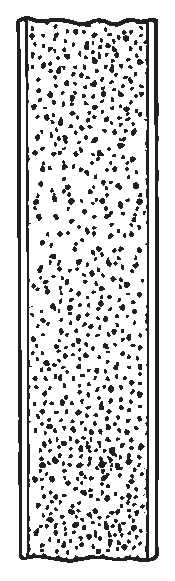
\includegraphics[width=.1\textwidth]{fig/fluidodinamica/vertical/ver-bubble.eps}} \label{fig:ver-bubble}} \quad
    \subfloat[][Flusso a slug]
    {\makebox[0.2\textwidth]{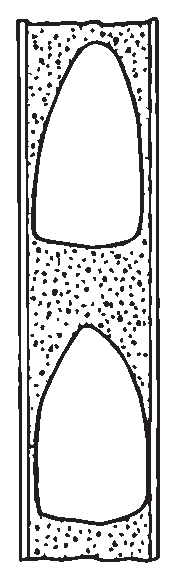
\includegraphics[width=.1\textwidth]{fig/fluidodinamica/vertical/ver-slug.eps}} \label{fig:ver-slug}}  \quad
    \subfloat[][Flusso a churn o agitato]
    {\makebox[0.2\textwidth]{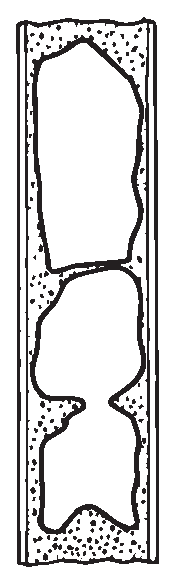
\includegraphics[width=.1\textwidth]{fig/fluidodinamica/vertical/ver-annular.eps}} \label{fig:ver-churn}} \quad
    \subfloat[][Flusso anulare misto]
    {\makebox[0.2\textwidth]{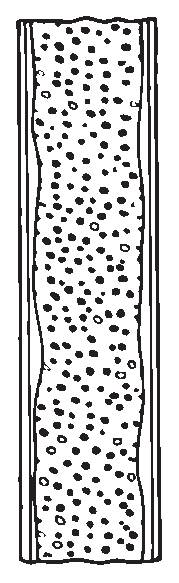
\includegraphics[width=.1\textwidth]{fig/fluidodinamica/vertical/ver-mist.eps}} \label{fig:ver-annular} }
\caption{Regimi di flusso bifase in condotte verticali}
\label{fig:verticale}
\end{figure}

Per comprendere nel dettaglio i vari regimi che si possono instaurare in condotta si fa riferimento alla mappa dei regimi di flusso bifase avvallata da \citeauthor{griffith1984multiphase} per condotte verticali (\figref{fig:ver-griffith}).

\begin{figure}[htbp]
    \centering
    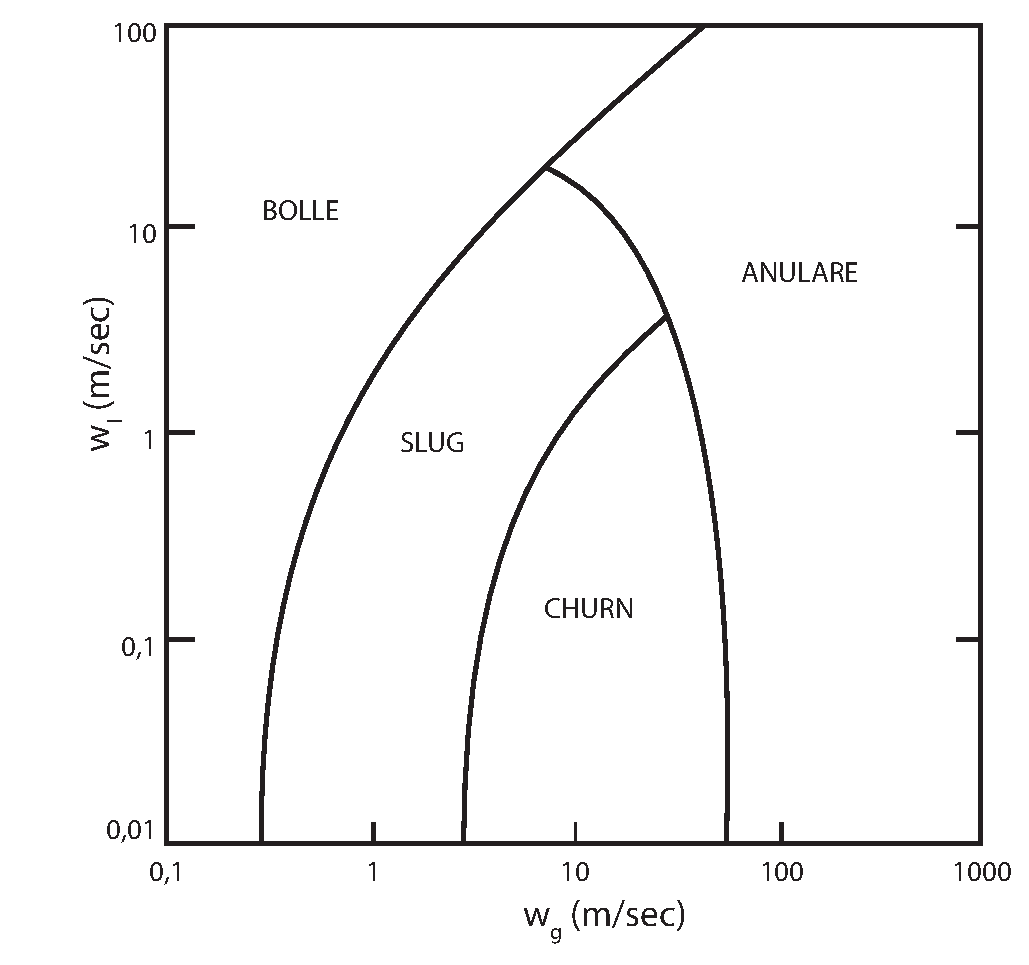
\includegraphics[width=.6\textwidth]{fig/fluidodinamica/ver-griffith.eps}
    \caption{Mappa per regimi di flusso bifase per condotte verticali \parencite{griffith1984multiphase}.}
    \label{fig:ver-griffith}
\end{figure}

Per basse velocità superficiali della fase gassosa, avviene in condotta il solo regime a bolle (\figref{fig:ver-bubble}). In questo regime la fase liquida si muove a velocità uniforme mentre le bolle di gas sono più veloci o più lente a seconda del loro diametro. Se si incrementa la velocità della fase gassosa, questa tenderà a viaggiare di pari passo alla fase liquida, creando così il regime a slug (\figref{fig:ver-slug}) e il regime a churn o anche detto agitato (\figref{fig:ver-churn}), dove ormai l'effetto della fase gassosa è predominante rispetto alla fase liquida. Nel regime anulare misto (\figref{fig:ver-annular}) la fase gassosa è continua e la fase liquida è dispersa nel gas oppure disposta sulle pareti interne.

\subsubsection{Condotte orizzontali}
I regimi di flusso in condizioni di condotta orizzontale possono essere così classificati (\figref{fig:orizzontale}):
\begin{itemize} 
    \item flusso stratificato;
    \item flusso a onde;
    \item flusso a plug o a bolle allungate;
    \item flusso a slug;
    \item flusso anulare;
    \item flusso a bolle disperse.
\end{itemize} 

\begin{figure}[htbp]
\centering
    \subfloat[][Flusso stratificato]
    {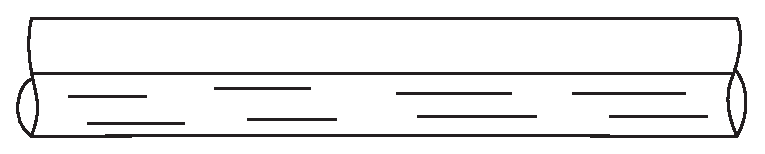
\includegraphics[width=.4\textwidth]{fig/fluidodinamica/horizontal/hor-stratified.eps} \label{fig:hor-stratified}} \qquad \qquad
    \subfloat[][Flusso a onde]
    {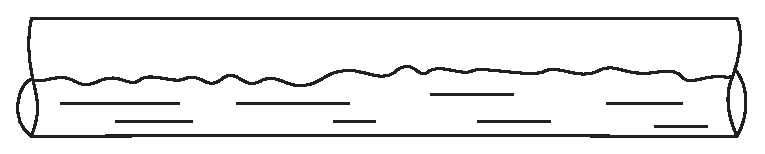
\includegraphics[width=.4\textwidth]{fig/fluidodinamica/horizontal/hor-wavy.eps} \label{fig:hor-wavy}} \\
    \subfloat[][Flusso a plug]
    {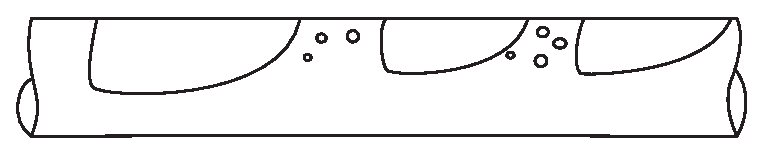
\includegraphics[width=.4\textwidth]{fig/fluidodinamica/horizontal/hor-plug.eps} \label{fig:hor-plug}} \qquad \qquad
    \subfloat[][Flusso a slug]
    {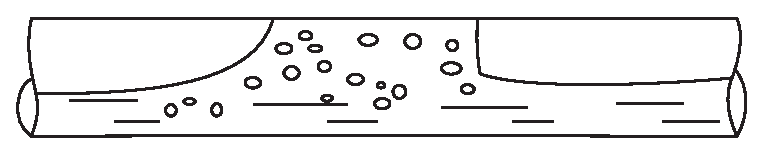
\includegraphics[width=.4\textwidth]{fig/fluidodinamica/horizontal/hor-slug.eps} \label{fig:hor-slug}}\\
    \subfloat[][Flusso anulare]
    {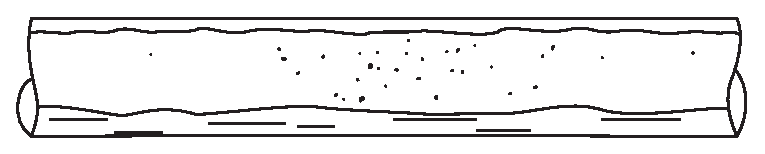
\includegraphics[width=.4\textwidth]{fig/fluidodinamica/horizontal/hor-annular.eps} \label{fig:hor-annular}} \qquad \qquad
    \subfloat[][Flusso a bolle disperse]
    {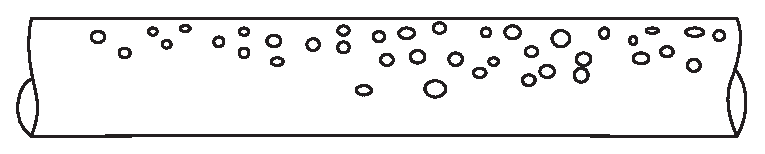
\includegraphics[width=.4\textwidth]{fig/fluidodinamica/horizontal/hor-bubble.eps} \label{fig:hor-bubble}}
\caption{Regimi di flusso bifase in condotte orizzontali}
\label{fig:orizzontale}
\end{figure}
Per la determinazione dei diversi regimi di flusso bifase aria-acqua si fa riferimento alle mappe per condotte orizzontali proposte da \textcite{griffith1984multiphase}, \textcite{baker1954simultaneous} e \textcite{taitel1976model}.

\paragraph{\textcite{griffith1984multiphase}}
Il regime di flusso è definito tramite la \textit{velocità superficiale} \(w_i\), legata alla portata volumetrica della fase i-esima attraverso una generica sezione \(A\) della condotta. Si ha quindi:
\[w_G = \frac{Q_G}{A} \addtag\]
\[w_L = \frac{Q_L}{A} \addtag\]
dove i pedici \(g\) e \(l\) fanno riferimento alla fase gassosa o liquida. Le linee continue interne rappresentano la transizione tra i diversi regimi.\\
Per basse velocità superficiali della fase liquida si verificano flussi stratificati a interfaccia liscia (\figref{fig:hor-stratified}), a onda (\figref{fig:hor-wavy})e anulare misto (\figref{fig:hor-annular}) a seconda della velocità superficiale del liquido. Questi tre regimi fanno parte della categoria dei flussi separati: le due fasi appaiono come due flussi continui senza apparente iterazione. Il flusso stratificato e quello a onde sono caratterizzati dallo scorrimento della fase liquida nella parte inferiore della condotta, in quello anulare la fase liquida si dispone lungo le pareti interne della condotta. All'aumentare della velocità superficiale della fase liquidi, si osserva un maggiore miscelamento delle due fasi e si verificano  flussi a slug o a bolle allungate (\figref{fig:hor-slug}) o flussi a plug (\figref{fig:hor-plug}). La differenza tra questi due regimi è sottile: nel flusso a slug sono disperse numerose bollicine di gas nella fase liquida, al contrario del flusso a plug. Ad alte velocità superficiali della fase liquida si verifica il flusso a bolle (\figref{fig:hor-bubble}), caratterizzato dalla presenza di bolle di gas disperse nella fase liquida.
\begin{figure}[htbp]
    \centering
    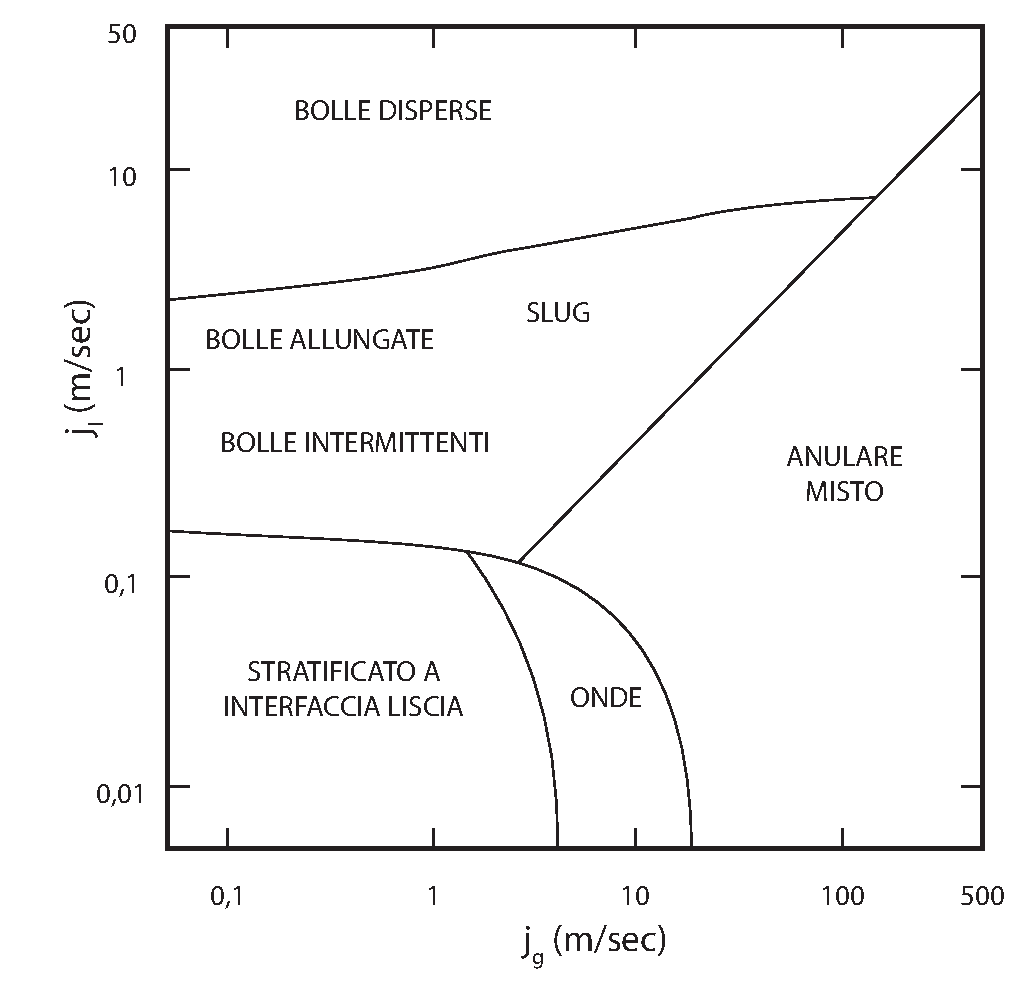
\includegraphics[width=.6\textwidth]{fig/fluidodinamica/hor-griffith.eps}
    \caption{Mappa di \textcite{griffith1984multiphase}) per regimi di flusso bifase per condotte orizzontali.}
    \label{fig:hor-griffith}
\end{figure}

\paragraph{\textcite{baker1954simultaneous}}
La mappa di \textcite{baker1954simultaneous} per condotte orizzontali con flusso bifase \figref{fig:baker} è stata proposta originariamente sia per Sistema Internazionale che per sistema consuetudinario statunitense. Per l'utilizzo della mappa devono essere determinati i parametri adimensionali \(\Lambda\) e \(\Psi\) e la \textit{velocità di massa} o \textit{flusso di massa} \(j_i\), la massa della fase i-esima che attraversa una generica sezione trasversale \(A\) della condotta:
\[j_G = \frac{\dot{m_G}}{A}=\frac{\rho_G w_G A}{A}=\rho_G w_G \addtag\]
\[j_L = \frac{\dot{m_L}}{A}=\frac{\rho_L w_L A}{A}=\rho_L w_L \addtag\]
dove \(j_G\) e \(j_L\) sono (in modulo) la velocità di massa del gas e del liquido. I parametri adimensionali \(\Lambda\) e \(\Psi\) sono definiti da:
\[\Lambda= \left(\dfrac{\rho_G}{\rho_{aria}} \dfrac{\rho_L}{\rho_{acqua}}\right)^{1/2} \addtag \label{eq:lambdabaker} \]
\[\Psi=\left( \frac{\sigma_{acqua}}{\sigma} \right) \left[ \left( \frac{\mu_L}{\mu_{acqua}} \right) \left( \frac{\rho_{acqua}}{\rho_L} \right)^2 \right]^{1/3} \addtag \]
dove \(\rho_G\), \(\rho_L\), \(\mu_L\) e \(\sigma\) sono proprietà proprie del fluido. I termini noti, quindi le proprietà di riferimento sono:
\begin{itemize}
    \item \(\rho_{acqua}=1000\) kg/m\ap{3};
    \item \(\rho_{aria}=1,23\) kg/m\ap{3};
    \item \(\mu_{acqua}=0,001\) N sec/m\ap{2};
    \item \(\sigma_{acqua}=0,072\) N/m.
\end{itemize}
I valori sugli assi x e y sono così identificati. L'intersezione sulla mappa fornisce il regime bifase che si instaura nella condotta sulla base del modello.
\begin{figure}[htbp]
    \centering
    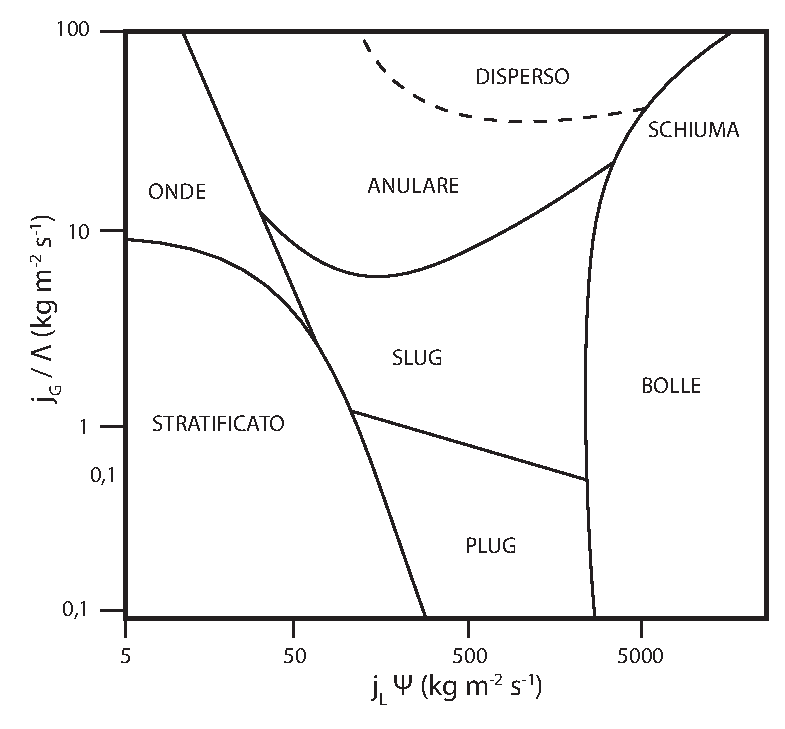
\includegraphics[width=.6\textwidth]{fig/fluidodinamica/baker.eps}
    \caption{Mappa di \textcite{baker1954simultaneous}) per regimi di flusso bifase per condotte orizzontali.}
    \label{fig:baker}
\end{figure}

\paragraph{\textcite{taitel1976model}}
Nel lavoto di \textcite{taitel1976model} (\figref{fig:taitel}) si propone una mappa per condotte orizzontali che nasce dalla combinazione di analisi analitiche e selezione empirica di numerosi parametri di riferimento. La mappa usa il \textit{parametro di Martinelli} \(\chi\), il \textit{numero di Froude} del gas \(Fr_G\) e i parametri \(T\) e \(K\).

\begin{figure}[htbp]
    \centering
    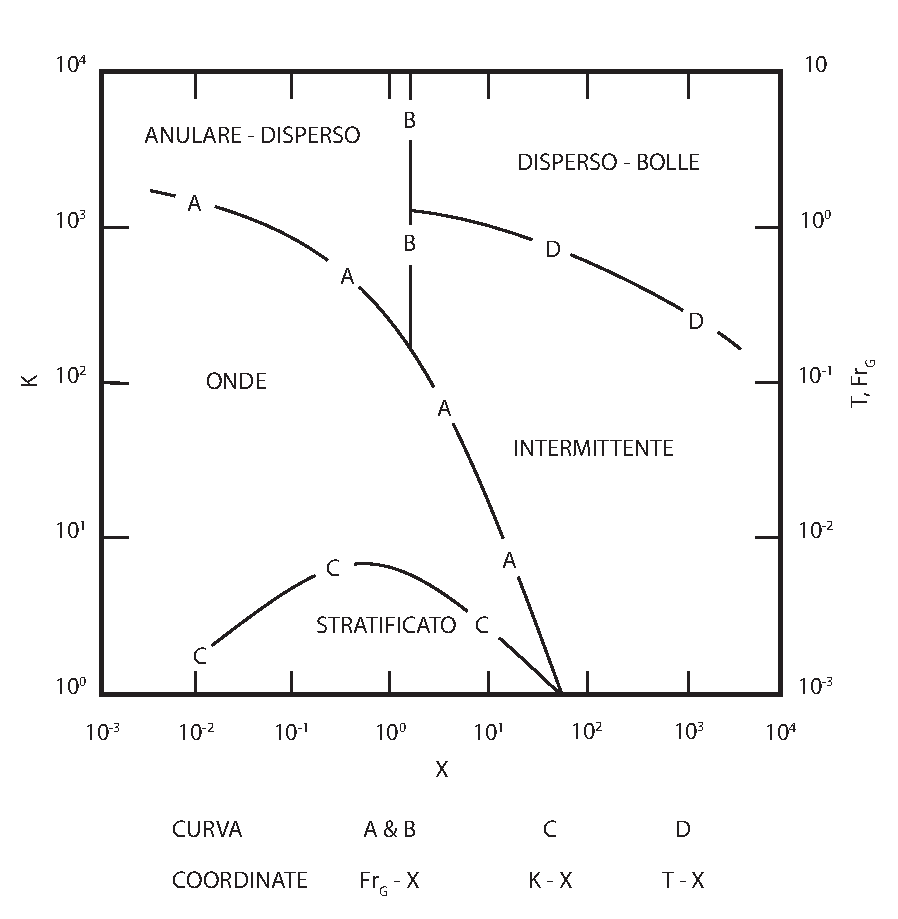
\includegraphics[width=.6\textwidth]{fig/fluidodinamica/taitel.eps}
    \caption{Mappa di \textcite{taitel1976model}) per regimi di flusso bifase per condotte orizzontali. Gli assi di riferimento cambiano a seconda della curva considerata, come descritto nel pannello al di sotto del grafico.}
    \label{fig:taitel}
\end{figure}

Il parametro di Martinelli è dato dalla radice quadrata del rapporto tra i gradienti di pressione del liquido e del gas:
\[\chi = \left[ \frac{(dp/dl)_L}{(dp/dl)_G} \right]^{1/2} \addtag \label{eq:martinelli} \]
Si ricorda che il gradiente di pressione per unità di lunghezza è dato dalla derivata dell'equazione di Darcy-Weisbach \eqref{eq:darcyweisbachP} in funzione della caduta di pressione lungo la direzione della condotta:
\[\Delta p_{a,k} = \lambda_k \; \frac{l}{D} \; \frac{\rho_k \; w_k^2}{2} \implies \left(\dfrac{dp}{dl}\right)_k =- \frac{\lambda_k}{D} \; \frac{\rho \; w^2}{2} = - \frac{\lambda_k \; j_k^2}{\rho_k \; D}  \addtag \label{eq:gradientepressione} \]
Il numero di Froude è un gruppo adimensionale e rappresenta la frazione liquida di un fluido.  Dal punto di vista analitico mette in relazione forza di inerzia con la forza peso. Per la fase gassosa vale:
\[Fr_G = \frac{j_G}{[\rho_G(\rho_L-\rho_G)D \; g]^{1/2}} \addtag \label{eq:froude}\]
Il parametro \(T\) è definito come:
\[ T = \left[ \dfrac{|(dp/dl)_L|}{g(\rho_L-\rho_G)} \right]^{1/2} \addtag \label{parametroT} \]
Il parametro \(K\) invece è funzione del numero di Froude del gas e del numero di Reynolds del liquido:
\[K=Fr_G \; Re_L^{1/2} \addtag \label{parametroK} \]
Caratteristica principale di questa mappa di regime è l'impiego di diverse coordinate, in funzione dei parametri trovati, a seconda della curva a cui si fa riferimento. Dapprima si calcolano quindi il parametro di Martinelli \(\chi\) e il numero di Froude del gas \(Fr_G\). Se le coordinate del punto trovato ricadono nella parte superiore della curva A, rappresentata rispetto al sistema di coordinate \(Fr_G-\chi\), il regime sarà quindi anulare. Nel caso in cui il punto si collochi al di sotto della curva viene calcolato il parametro \(K\). Facendo riferimento alla curva C e quindi al sistema di coordinate \(K-\chi\) il regime sarà a onde o stratificato con interfaccia liscia se il punto trovato è rispettivamente nella parte superiore o inferiore della curva C. Se il punto ricade nella parte superiore a destra del grafico, si fa riferimento alla curva D, quindi al sistema di coordinate \(T - \chi \). Il regime sarà a bolle disperse se il punto trovato si trova al di sopra della curva D, viceversa il regime sarà di natura intermittente o a slug. \\ \\
Tutti i modelli fin qui presentati sono stati sviluppati per flussi bifase in condizioni adiabatiche. Tuttavia questi modelli, tramite accorgimenti di natura analitica, posso risponde anche a condizioni diabatiche, cioè ipotizzando la condotta come sistema aperto in cui avviene scambio di calore con l'esterno. Lo studio dei regimi di flusso può quindi essere esteso, per esempio, negli impianti di refrigerazione oppure negli scambiatori termici.

\subsection{Cadute di pressione per attrito di un flusso bifase}
Si può semplificare lo studio del moto di un fluido bifase se si assume che le fasi siano ben miscelate fra loro, quindi come un unico fluido monofase. Il \textit{modello omogeneo} può essere applicato quando le fasi sono fortemente interdisperse tra loro, cioè quando entrambe le fasi hanno velocità superficiali sostenute. Le perdite di carico totali \(\Delta p_{tot}\) sono la somma delle perdite di carico statiche o gravitazionali \(\Delta p_s\), le perdite di carico della quantità di moto \(\Delta p_{mom}\) e le perdite di carico per attrito \(\Delta p_a\): 
\[\Delta p_{tot} = \Delta p_s +\Delta p_{mom} + \Delta p_a \addtag \label{eq:perditetot}\]
La perdita di carico statico per un fluido bifase omogeneo è:
\[\Delta p_s = \rho_H \; g \; z\ \addtag \]
dove \(z\) è la differenza di quota geodetica tra le sezioni di ingresso e uscita della condotta, o meglio l'altezza della condotta. Per densità omogenea \(\rho_H\) si intende:
\[\rho_H=\rho_L(1-\epsilon_H)+\rho_G \; \epsilon_H \addtag \label{eq:omogenea} \]
Si determina la frazione di vuoto \(\epsilon_h\) in funzione del titolo di vapore \(x\):
\[\epsilon_H = \left[ 1+ \left( \dfrac{w_G}{w_L} \dfrac{(1-x)}{x} \dfrac{\rho_G}{\rho_L} \right) \right]^{-1} \addtag \]
dove il rapporto \(w_G/w_L\) è detto \textit{rapporto di slittamento} e ha valore unitario nel caso di flussi omogenei. Il gradiente di pressione della quantità di moto per unità di lunghezza del condotto è:
\[\left( \dfrac{dp}{dl} \right)_{mom}=\dfrac{d(j_{tot}/\rho_H)}{dz} \addtag \]
Il punto cruciale del calcolo delle cadute di pressione per un flusso bifase risiede nella stima del termine di attrito, in questo frangente rappresentato dal numero di Fanning \(f\). Se si esprime la \eqref{eq:darcyweisbachP} in funzione del numero di Fanning \(f_{tot}\) per un flusso bifase, in funzione del flusso di massa \(j_{tot}\):
\[\Delta p_a = \dfrac{2 \; f_{tot} \; j_{tot}^2}{\rho_{tot}} \; \dfrac{l}{D} \addtag \label{eq:darcyweisbachfanning2f} \]
Si può esprimere il numero di Fanning tramite la \eqref{eq:fanningreynolds}, il numero di Reynolds per mezzo della \eqref{eq:reynolds}. Come viscosità, parametro utile al calcolo del numero di Reynolds, può essere scelta quella della fase liquida oppure una media pesata in base al titolo di vapore \(x\):
\[\mu_{tot} =x \; \mu_G + (1+x) \; \mu_L \addtag \]
\\
\'E importante acquisire le basi della fluidodinamica multifase per capire come le iterazioni tra le diverse fasi e le perdite di carico definiscano il flusso che si instaura in condotta. L'ingegneria petrolifera ha affinato negli anni i modelli interpretativi, così da avvicinare le stime di produzione di un pozzo ai trend reali. In particolar modo, la corretta interpretazione del moto multifase per i pozzi a gas determina la tipologia e la configurazione di sistemi per l'aumento di portata o la diminuzione delle perdite di carico. Si intuisce quindi che l'aumento delle performance è legato alla veridicità del modello calcolato. Nel prossimo capitolo sono trattati i problemi di un pozzo a gas legati a condizioni di flusso multifase e le tecnologie oggi utilizzate per ovviare al calo di rendimento nel tempo.
%\section{Moto dei fluidi comprimibili in condotta a sezione variabile}
%\subsection{Velocità del suono}
%\subsection{Equazione di Hugoniot e numero di Mach}
%\subsection{Propagazione dei disturbi in flussi subsonici e supersonici}
%\subsection{Proprietà al ristagno}
%\subsection{Flusso attraverso un'onda d'urto normale}

